\begin{center}
  \textbf{Exercices Matlab - Analyse Numérique - 2017 \\
  Section MA \\
  Prof. A. Quarteroni \\
  Séance 1 - Introduction à Matlab}
\end{center}


\vspace{10mm}

\textbf{Exercice 1 \\}
On considère les matrices
\begin{equation*}
  A = \begin{bmatrix}
        5 & 3 & 0  \\
        1 & 1 & -4 \\
        3 & 0 & 0
      \end{bmatrix}
  , \quad 
  B = \begin{bmatrix}
        4 & 3 & 2  \\
        0 & 1 & 0  \\
        5 & 0 & 1/2
      \end{bmatrix}
\end{equation*}


Créer un répertoire de travail et écrire un fichier ".m" dans lequel placer les instructions pour calculer (sans utiliser de boucles), la matrice $C = AB$ (produit matriciel) et la matrice $D$ qui a comme éléments $D_{ij} = A_{ij} B_{ij}$ (produit composante par composante).






\textbf{Solution 1 \\}
Dans le script \texttt{ex1.m}, nous avons :
\lstinputlisting{s1/matlab/ex1a.m}

On obtient
\lstinputlisting{s1/matlab/ex1b.m}



\textbf{Exercice 2 \\}
Définir (sans utiliser de boucles) la matrice diagonale de taille $n = 5$ dont la diagonale est un vecteur de points équirépartis entre $3$ et $6$ (i.e. $\squared{3, 3.75, 4.5, 5.25, 6}$).


\textbf{Solution 2 \\}
\lstinputlisting{s1/matlab/ex2.m}


\textbf{Exercice 3 \\}
Écrire une fonction pour calculer :
\begin{enumerate}
  \item le produit, composante par composante, entre deux vecteurs $x$ et $y$ ;
  \item le produit scalaire entre les mêmes vecteurs $x$ et $y$ ;
  \item un vecteur dont les éléments sont définis par : \\
        $v_1 = x_{1} y_n, \quad
        v_2 = x_2 y_{n-1}, \quad
        \dots, \quad
        v_{n-1} = x_{n-1} y_2, \quad
        v_n = x_n y_1.$
\end{enumerate}


Utiliser et compléter la définition suivante :
\lstinputlisting{s1/matlab/ex3.m}

Tester la fonction avec \MAT.



\textbf{Solution 3 \\}
\lstinputlisting{s1/matlab/operations.m}
\lstinputlisting{s1/matlab/ex3out.txt}


\textbf{Exercice 4 \\}
En utilisant la commande \texttt{diag}, définir en \MAT la matrice $A \in \R^{n \times n}$ avec $n = 10$

\begin{equation*}
  \begin{bmatrix}
      2   & -1  &         &         &         &    \\
      -1  & 2   & -1      &         &         &    \\
          & -1  & 2       & -1      &         &    \\
          &     & \ddots  & \ddots  & \ddots  &     \\
          &     &         &         &         &    \\
          &     &         &         &    -1   &  2  
    \end{bmatrix}
\end{equation*}


Ensuite, calculer les quantités suivantes :
\begin{enumerate}
  \item le déterminant de $A$ ;
  \item les normes $\norm{A}_{1}$, $\norm{A}_{2}$, $\norm{A}_{\infty}$ (tapez \texttt{help norm} pour voir les options) ;
  \item le rayon spectral de $A$, noté $\rho \parent{A}$. On rappelle que $\rho \parent{A} = \max_{j = 1, \dots, n} \abs{\lambda_{j} \parent{A}}$, ou $\lambda_{j} \parent{A}$ sont les valeurs propres de $A$. Vérifier que, puisque $A$ est symétrique et définie positive, on a $\rho \parent{A} = \norm{A}_{2}$ ;
\end{enumerate}

Visualiser les vecteurs propres $\mathbf{v}_{j}, j \in \bracket{1, \dots, 10}$ en utilisant les commandes \texttt{[v, lambda]=eig(A)} et \texttt{plot(v)}.


En utilisant \MAT, vérifier que la matrice $V$ (dont les colonnes sont égales aux vecteurs propres de $A$) permet de diagonaliser la matrice $A$. En particulier, vérifier que
\begin{equation*}
  V^{-1} A V = D = \text{diag} \bracket{\lambda_{1}, \dots, \lambda_{n}}.
\end{equation*}


Visualiser finalement la structure des matrices \texttt{A}, \texttt{V}, \texttt{D} (avec la commande \texttt{spy}).



\textbf{Solution 4 \\}
On peut définir la matrice $A$ avec la commande suivante

\begin{verbatim}
n=10;
A=2*diag(ones(1,n))-diag(ones(1,n-1),1)-diag(ones(1,n-1),-1);
A
\end{verbatim}

Après, on calcule son déterminant par

\begin{verbatim}
det(A)

ans = 11
\end{verbatim}

et les normes $\norm{A}_{1}$, $\norm{A}_{2}$, $\norm{A}_{\infty}$ par

\begin{verbatim}
nrm1=norm(A,1)
nrm2=norm(A,2)
nrminf=norm(A,inf)
\end{verbatim}

et on obtient

\begin{verbatim}
nrml = 4
nrm2 = 3.9190
nrminf = 4
\end{verbatim}


Pour évaluer le rayon spectral de $A$, il faut calculer ses valeurs propres et en prendre le maximum, en valeur absolue :
 
\begin{verbatim}
rho=max(abs(eig(A)))

rho = 3.9190
\end{verbatim}
 
On peut directement vérifier que, $A$ étant symétrique et définie positive, on a $\rho \parent{1} = \norm{A}_{2}$.
Pour calculer et visualiser les vecteurs propres $\BoldV_{j}, j \in \bracket{1, \dots, 10}$, il faut utiliser les commandes

\begin{verbatim}
[V, D]=eig(A);
figure
plot(V)
\end{verbatim}


ou, si on veut visualiser chaque vecteur propre individuellement, la boucle suivante :
 
\begin{verbatim}
figure
for i=1:10
    plot(V(:,i))
    pause
end
\end{verbatim}

Avec la première option, on a le graphe de la Figure \ref{fig:comp}.

\begin{figure}[h!]
  \centering
  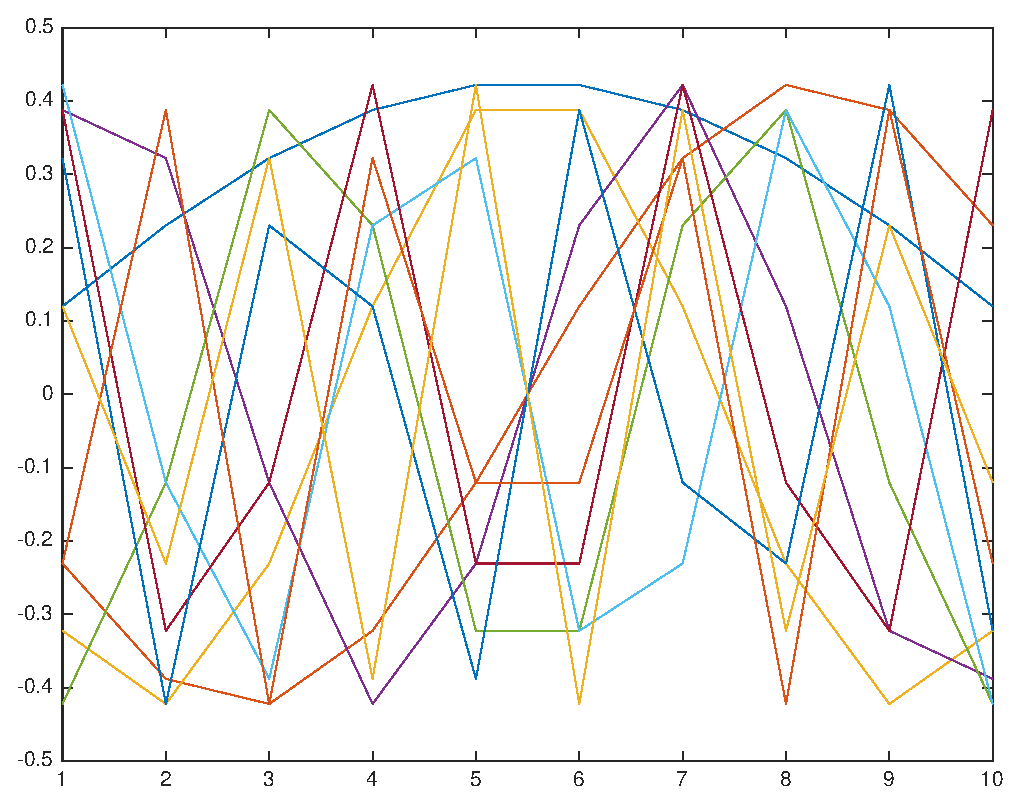
\includegraphics[scale = 0.5]{s1/matlab/comp.eps}
  \caption{Composantes des vecteurs propres de la matrice $A$.}
  \label{fig:comp}
\end{figure}


Pour vérifier que la matrice $V$ (dont les colonnes sont égales aux vecteurs propres de $A$) permet de diagonaliser la matrice $A$, c'est-à-dire $V^{-1} A V = D = \text{diag} \bracket{\lambda_{1}, \dots, \lambda_{n}}$, il faut utiliser les commandes suivantes :


\begin{verbatim}
[V,D]=eig(A)
inv(V)*A*V % ou mieux (V\A)*V
D
dif = norm(D-inv(V)*A*V); % ou mieux dif = norm(D-(V\A)*V);
\end{verbatim}

on obtient

\begin{verbatim}
dif = 3.5003e-15
\end{verbatim}

Enfin, pour visualiser la structure des matrices \texttt{A}, \texttt{V}, \texttt{D}, il faut taper

\begin{verbatim}
spy(A)
spy(D)
spy(V)
\end{verbatim}

On peut observer à la Figure \ref{fig:structure} que la matrice $A$ est tri-diagonale, la matrice $D$ est diagonale alors que la matrice $V$ des vecteurs propres est pleine : tous ses éléments sont différentes de zéro.

 





\begin{figure}[h!]
  \begin{subfigure}[b]{0.3\linewidth}
    \centering
    \includegraphics[scale=0.2]{s1/matlab/A} 
    %\caption{Interpolation of $f$ using NCS \\ with $7+2$ points} 
    %\label{fig:q11_n7} 
  \end{subfigure}
  \begin{subfigure}[b]{0.3\linewidth}
    \centering
    \includegraphics[scale=0.2]{s1/matlab/D} 
    %\caption{Interpolation of $f$ using NCS \\ with $8+2$ points} 
    %\label{fig:q11_n8} 
  \end{subfigure}
  \begin{subfigure}[b]{0.3\linewidth}
    \centering
    \includegraphics[scale=0.2]{s1/matlab/V} 
    %\caption{Interpolation of $f$ using NCS \\ with $8+2$ points} 
    %\label{fig:q11_n8} 
  \end{subfigure} 
  \caption{Structure des matrices $A$, $D$ et $V$ de gauche à droite.}
  \label{fig:structure}
\end{figure}




\textbf{Exercice 5 \\}
\begin{enumerate}[label=\alph*)]
  \item Soit
  
  \begin{equation*}
    f \parent{x} = \dfrac{x^{2}}{2} \sin \parent{x}, 
    \quad x \in \squared{1, 20}
  \end{equation*}
  
  une fonction qu'on veut représenter graphiquement en choisissant 10 points, 20 points et 100 points dans l'intervalle de définition. Écrire un fichier ".m" pour réaliser les trois graphiques sur la même figure et avec trois couleurs différentes. Quelle est la meilleure représentation ?
  
  \item Faire la même chose pour les fonctions :
  
  \begin{equation*}
    g \parent{x} = \dfrac{x^{3}}{6} \cos \parent{\sin \parent{x}} \exp{-x} + \parent{\dfrac{1}{1+x}}^{2}, 
    \quad x \in \squared{1, 20}
  \end{equation*}
  
  \begin{equation*}
    h \parent{x} = x \parent{1 - x} + \dfrac{\sin \parent{x} \cos \parent{x}}{x^3},
    \quad x \in \squared{1, 20}
  \end{equation*}
\end{enumerate}





\textbf{Solution 5 \\}
\begin{enumerate}[label=\alph*)]
  \item Le script \texttt{ex5.m} est 
  
  \lstinputlisting{s1/matlab/ex5.m}
  
  \begin{figure}[h!]
    \centering
    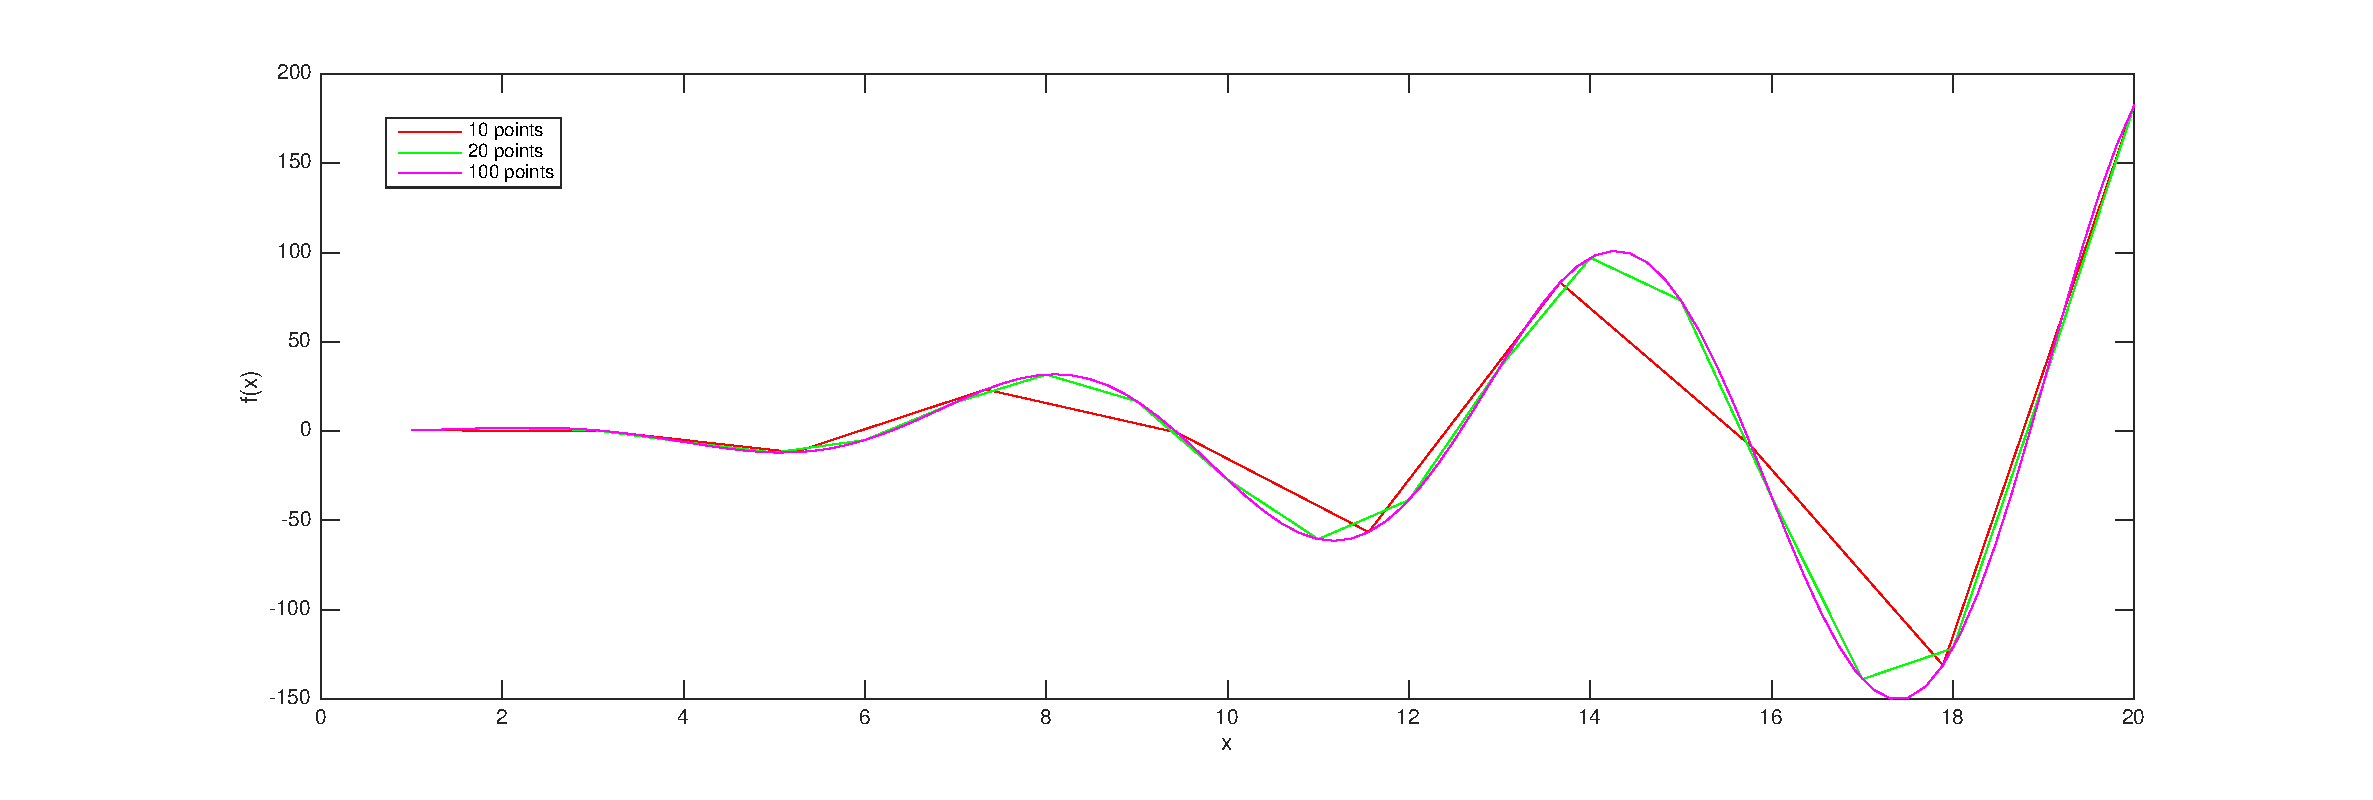
\includegraphics[scale = 0.4]{s1/matlab/f5.eps}
    \caption{Graphe de la fonction $f$.}
    \label{fig:f5}
  \end{figure}

  
  \item On remplace la fonction $f$ par les fonctions $g$ et $h$ :
  
  \lstinputlisting{s1/matlab/ex5gh.txt}
\end{enumerate}


